\chapter{Wireless Sharing and Access Control}\label{waccess}\index{Access control}

\minitoc 

\clearpage
\section*{Objectives}
To develop an understanding of:
\begin{itemize}

\item how nearby wireless devices are able to share access to spectrum;

\item the CSMA/CA multiple access scheme;

\item how devices are able to co-exist by treating nearby signals as noise;

\item the alternative spectrum sharing technologies that are available.

\end{itemize}

\section{Carrier Sense Multiple Access (with Collision Avoidance)}\index{CSMA/CA}\label{CSMA/CA}

Carrier-sense multiple access with collision avoidance (ie; CSMA/CA) is a
medium access control protocol developed for IEEE 802.11 wireless local
area networks.  This method is used to assist with collision avoidance
in wireless networks, where multiple wireless devices connected to the
wireless network can "see" access points forming part of the wireless
network but not other wireless devices.

In early versions of wired Ethernet networks adopted the carrier-sense
multiple access with collision detection (CSMA/CD) protocol to allow the
orderly transmission of data across the network. In wireless networks, it
is harder for a device to detect collisions taking place so an
avoidance method is adopted which aims to prevent any collisions
happening in the first place.

Some of the reasons for the difficulty in detecting collisions include
differences in transmit power level, the receive sensitivity, the
range and location of the device with respect to the access point. These
factors may cause an access point to not be able to ``hear" another access
point's broadcast. This condition in a wireless network is referred to as
``hidden node".

The high level sequence of hand shakes between the device and the access
point takes place when a device is  prepared to send data over a wireless
network, with CSMA/CA capability enabled. The communication hand shaking
between the device and access point include:

\begin{enumerate}[(i)]

\item When a device is about to send data, it check that the communications 
channel is ``idle" and sends out a request to send (RTS)\index{RTS} message to the ``seen" access point/s.
\item The access point receives the RTS message and if there's no other 
simultaneous data communications taking place by other connected devices, 
it sends the device a clear to send (CTS)\index{CTS} message.
\item In the case the access point receives the RTS message and simultaneous 
data communications is taking place between other devices (ie a risk of collision 
exists), then no CTS message is sent to the waiting device.
\item After a random wait time generated by the device lapses, the 
device will re-send the RTS to the access point/s.
\item This process is repeated until a free communications channel is 
available and a CTS message is received from the access point.

\end{enumerate}

\begin{figure}
\centering
	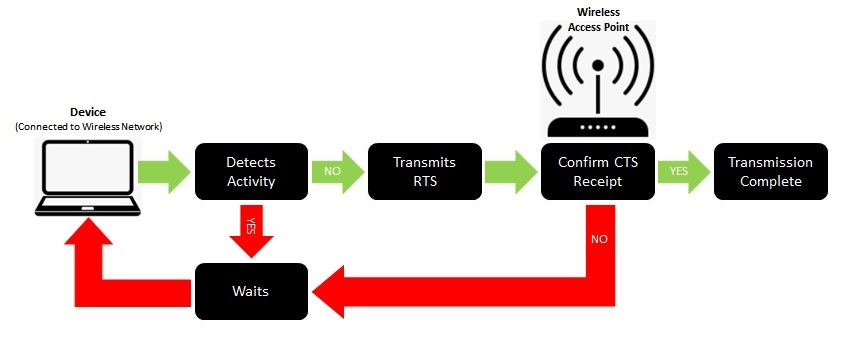
\includegraphics[width=12cm]{CSMA_CA.jpg}
	\caption{CSMA/CA Data Message Transmission Process}
	\label{CSMA_CA}
\end{figure}



\section{MAC Sub-Layers}

IEEE 802.11 defines two medium access control (ie; MAC) sub-layers, namely:
\begin{enumerate}[(i)]
\item The mandatory Distributed Coordination Function (DCF), and
\item The optional Point Coordination Function (PCF).
\end{enumerate}

\begin{figure}
\centering
	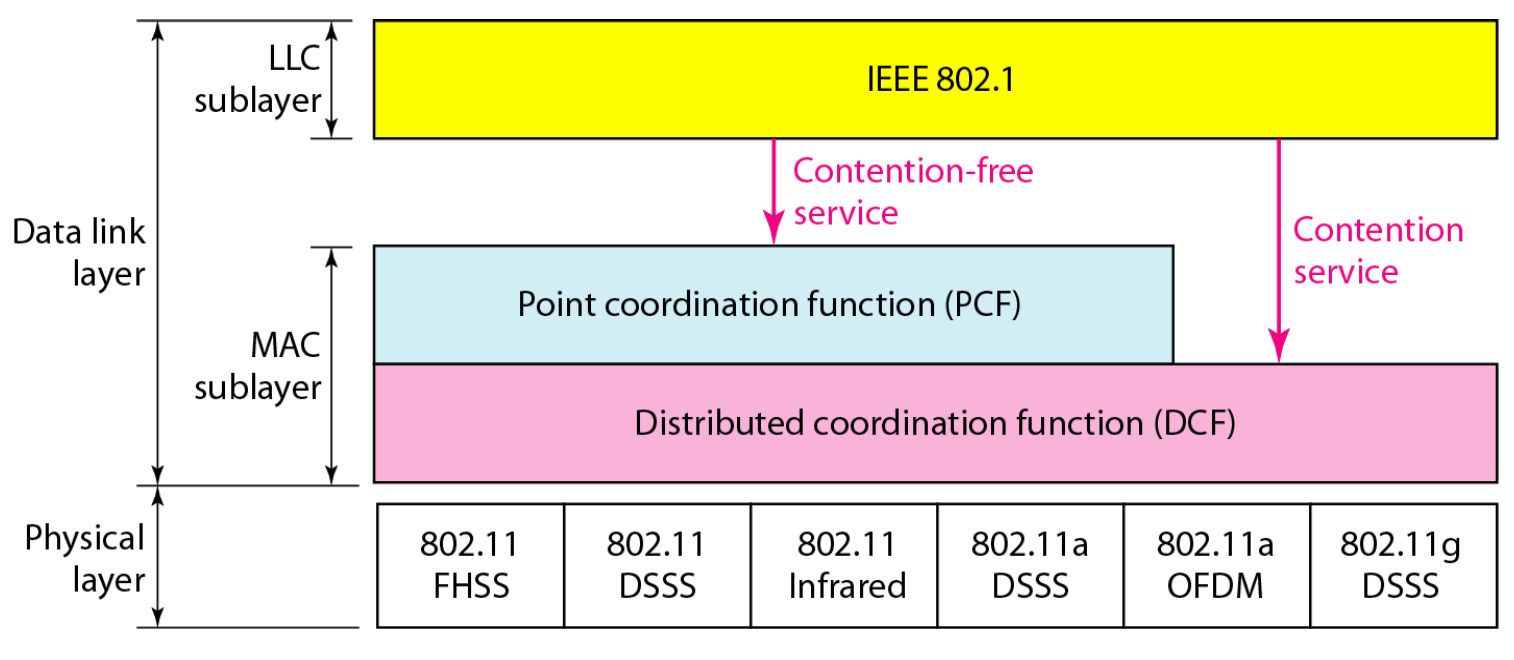
\includegraphics[width=12cm]{mac_layers.png}
	\caption{DCF and PCF MAC Sub-Layers}
	\label{CSMA_CA}
\end{figure}



\section{Sharing by Treating Other Channels as Noise}\label{sharingasnoise}


Treating other nearby devices as background noise happens automatically, if they are sufficiently far away,
and consequently it is not usually regarded as a {\em method} for sharing spectrum.
Nevertheless, if one pair of devices are located within close proximity to each other,
and a second pair of devices are also mutually close to each other, but the first pair
is somewhat further from the second pair, than the distances within the pair,
the signal from one pair to the other will be relatively so weak that it will not be detectable, and will
be ignored (except that the estimation of background noise power will include noise due to 
other devices). 
The two pairs of devices can share the same spectrum, without causing significant
interference to each other. In this arrangement, one pair's signal appears to the others 
as {\em noise}.

Although this type of sharing happens automatically, and the only technical work required
to take advantage of it is to constantly measure the signal to noise ratio, which all wireless
devices are {\em already doing}, it is not the case that this sharing mechanism is unimportant or
ineffective. To the contrary, this method of sharing of spectrum is probably the most important
we have.

Here is an analogy: suppose, instead of wireless spectrum, we are considering how to manage 
water supply. This is achieved by means of dams, catchments, pumping stations, reticulation networks.
And, don't forget: {\em rainfall}! In fact, rainfall (and the whole water cycle of the earth) 
does 99\% of the work for us, with almost no design or management by the human population.

In the same way, it is really the inverse square law (see \S\ref{powervsdistance}) which 
does 99\% of the work towards efficient and reliable sharing of spectrum.

There are some techniques that we can use to take better advantage of this mechanism:
in particular, this is why wireless access points should not be located too close
to each other. In addition, when two wireless access points are close enough
to cause interference to each other, this interference can be reduced by 
configuring them to use different {\em channels}. The term {\em channel}\index{channel} is
used in the field of communication to mean any end-to-end medium, but in 
802.11, in particular, it has been assigned a more specific meaning. A channel
is an allocation of spectrum. The channel spectrum allocations are not
{\em disjoint}, i.e. there is some overlap between nearby channels, and
especially between adjacent channels.\index{channel!non-overlapping}

If nearby wireless access points are assigned {\em adjacent} channels
they will interfere with each other, reducing throughput. This seems a bit disturbing,
at first sight. For this reason, it is recommended to assign channels to wireless
access points in such a way that nearby access points do not use nearby channels.

However, the problem of interference from nearby access points is not necessarily
as bad as at first sight because in these situations the communicating devices
will benefit from their physical separation {\em in addition} to the lowering
of signal power due to the channel separation, even when the channels are not
completely disjoint.

\section{Code Sharing}\index{code sharing}

Rather than carving up capacity for each user by allocating spectrum, or 
allocating a {\em time} for each pair of devices, 
we can also assign each pair of devices a {\em code}. In CSMA/CA (see \S\ref{CSMA/CA}),
all users share the same channel, and each user transmits data
in a burst which contains a packet. In effect, each pair of devices is
allocated its own {\em time}, for using the channel. This is called contention-based 
access. 

In addition to separating communications over common spectrum by frequency,
or by time, we can also separate them by {\em code}. 

\subsection{Direct Sequence Spread Spectrum}
	  		
In Direct Sequence Spread Spectrum\index{Direct Sequence Spread Spectrum} 
(DSSS)\index{DSSS}, each bit in the original signal is encoded as multiple
bits in the transmitted signal by using a {\em spreading code}\index{code!spreading}. 
Each transmitted bit is called a chip\index{chip}. The chipping
code is the code used to spread the signal across a wider frequency band in direct proportion to the number
of bits used. Then, a 10-to-1 chipping code spreads the signal across a frequency band that is 10 times
greater than a 1-bit chipping code. 

Figure \ref{DSSS} shows and example of DSSS. The original signal
(Data input A in the figure) is combined with the chipping code (PN bit stream in the figure) by using
an exclusive-OR (XOR). The XOR function will return a '0' if the two combined bits are equal, for example
'0' and '0' or '1' and '1', and will return a '1' if the two combined bits are different. The transmitted signal
is a combination of the original signal and the spreading code sequence. It has a wider bandwidth
than the original information signal. The example shows a 4-to-1 chipping code.
	  		
\begin{figure}
\begin{center}
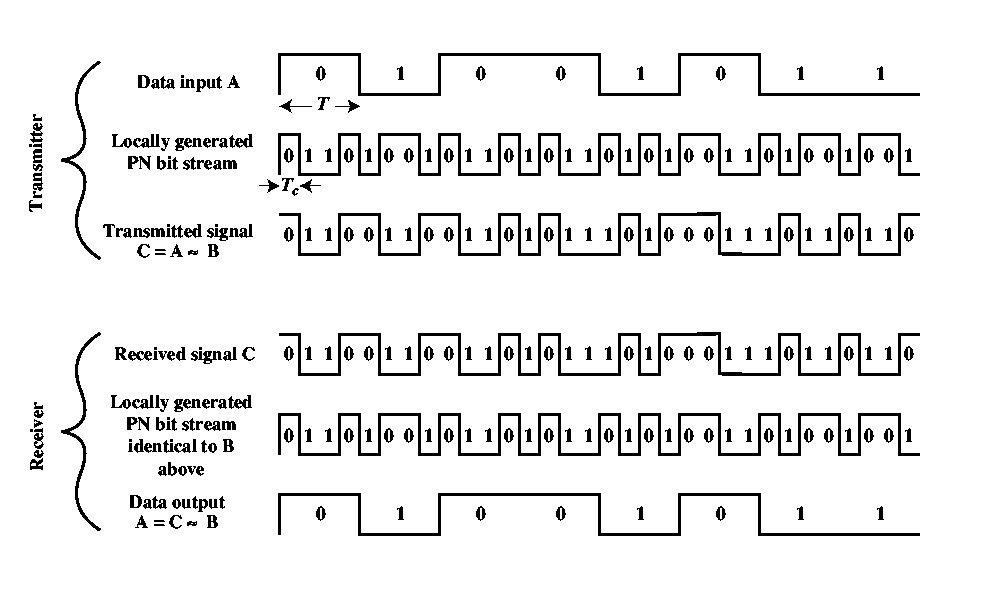
\includegraphics[width=15 cm]{DSSS.jpg}
\caption{Example of Direct Sequence Spread Spectrum [from W. Stallings]}\label{DSSS}
\end{center}
\end{figure}

A DSSS signal is very resilient to interference, which means that the transmitted signal can 
lose several chips (bits) in a word before the encoded data bit is corrupted. Additionally, DSSS allows
multiple users to share the same bandwidth, just by simply using different chipping sequences. 


\begin{exercise}{Direct Sequence Spread Spectrum}
Consider a DSSS system which uses the codes \verb|00000000| and \verb|11111111| for
one pair of users and the codes \verb|01010101| and \verb|10101010| for the other pair of users.
Now suppose the received signal is:
\begin{verbatim}
01010101121212121010101000000000
\end{verbatim}
Decode this signal, i.e. work out what are the messages being sent by each pair of users
to each other. Observe that decoding the messages presumes that we know where the
boundary between transmitted symbols lies. How could the boundary be determined
by a receiver, purely by observing the signal received?
\end{exercise}


\begin{sbexample}{Modelling CDMA with a spreadsheet}%
Read the example in \cite{cdmawiki}. A spreadsheet for doing all the
calculations in this example has been prepared and is shown in Figure
\ref{cdmaspread}. This spreadsheet can be downloaded from the course
web page. Try changing the messages which are encoded, checking that
the messages are always correctly decoded.

\begin{figure}
\begin{center}
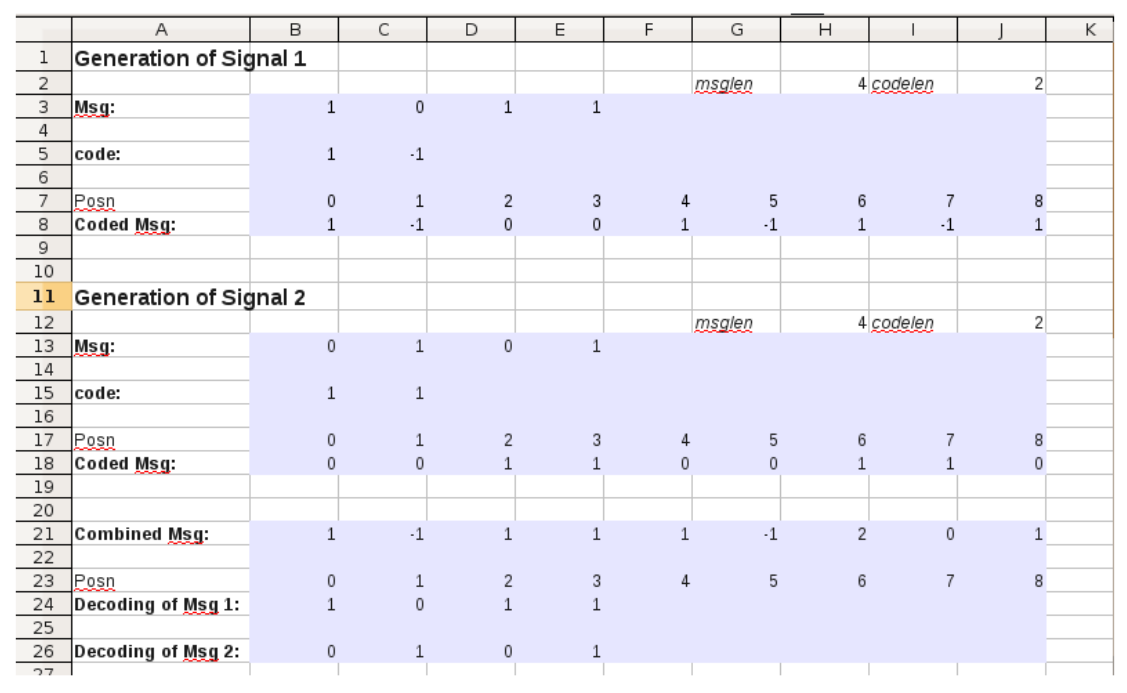
\includegraphics[width=15 cm]{cdmaspreadsheet.png}
\caption{Direct Sequence Spread Spectrum Coding in a Spreadsheet}\label{cdmaspread}
\end{center}
\end{figure}
\end{sbexample}

\begin{exercise}{Wireless communication modelled by a spreadsheet}
Starting with the second coding spreadsheet available from the course
web site, the one called \verb|coding2.xls|, construct a model of a
DSSS system which uses 6 orthogonal codes. The following eight codes
are orthogonal (see \cite{wolframwalsh}) so any six of these codes can
be used:

\begin{verbatim}
11111111
11110000
11000011
11001100
10011001
10010110
10101010
\end{verbatim}

\end{exercise}

\subsection{Power and CDMA}\index{CDMA}
Prior to the introduction of CDMA for access management, cellular
phones used FDMA, TDMA, or a combination of FDMA and TDMA for
separating the transmissions of different mobile devices in the same
cell. CDMA for mobile phones was introduced by Qualcomm in the U.S. in
1990 \cite{qualcommwiki}. It was immediately recognised that CDMA has
considerable advantages in this application, and many systems developed
since have used CDMA as a multiple access management method.

The reason probably relates mainly to the great ease with which CDMA
systems are able to recognise and respond to the impact of transmissions
to and from other mobile phones in the same or adjacent cells. In a CDMA
system all the phones sharing the same bandwidth, but using different
spreading codes, are perceived as generating additional background noise.
The amount of this noise depends not just on the number of other phones,
but also on how close they happen to be, and how much power they are
using. A phone which is a long way away, and transmitting at a low level
(because it is close to the base station, for example) will have a much
lower impact than one which is nearby and transmitting at maximum power.

In systems which use frequency and time to separate the transmissions
of different devices, there is no scope to take advantage of the fact
that sometimes the configuration of devices works in our favour, and so,
in effect, the bandwidth has to be sub-divided to suit the worst case
(where the phones are clustered near to each other, and all are a long
way from the base station). Although it is true that a system which
uses FDMA and/or TDMA to separate the communications of all the devices
in a cell will continue to operate well even when all the devices are
clustered together, in a sense this can now be seen, given the option
of using CDMA, as an excessively conservative design.


\section{OFDMA}\index{OFDMA}

Wireless transmission has evolved dramatically in the last two decades, to the point where
most of us use several wireless devices many times each day. One of the most difficult
problems facing designers of wireless channels at the start of this revolutionary development
phase was the problem of multipath transmission. In almost every application of wireless
that we engage in, during a typical day, there are multiple communication paths between the
mobile device that we are using and the antenna with which it is communicating.

These multiple paths do not naturally reinforce each other at the receiver. In rare cases, in
fact, the signals between two paths interfere with each other in such a way that they cancel
each other. In general the signal which results from the aggregation of the different paths will
look quite different from the one which was sent.

Orthogonal Frequency Division Multiplexing (OFDM) \cite{LiStuber2006} was invented more than forty
years ago, however it did not come into widespread use until recently. This long delay was
due to the fact that implementation of OFDM has been made relatively cheaper and more
straightforward by the development of high speed digital signal processing hardware which
was not available earlier.

Although it has taken a long time to become attractive, OFDM is now the preferred tech-
nology for modulating a digital signal onto a high frequency wireless or wired carrier in the
most important communication systems in use today: WiFi, ADSL, and mobile phones.

OFDM is not really a multiplexing system. The term muliplexing occurs in its name because
it can be viewed as the following strategy: sub-divide the signal to be transmitted into N
sub-signals (e.g. the first sub-signal is obtained by taking the first byte out of every N, the
second by taking the second byte, and so on). The sub-signals are then multiplexed onto the
channel by using N separate bands separated by frequency.

These $N$ frequency bands are packed very closely together. Normally, when two signals are
modulated onto a carrier in adjacent frequency bands they will overlap, in frequency, and
cause interference with each other. In OFDM, the way in which the side-by-side bands are
used ensures that there is no interference. This is the meaning of the term orthogonal.

This approach for sub-dividing and managing the available bandwidth has some inherent
advantages. In particular, each of the overlapping sub-bands is much narrower than the whole
band. Each sub-band has a guard band on either side, of frequencies where the signal leaks
out to other frequencies, which therefore can’t be used. Because of orthogonality there is
no need for these guard-bands to be unused between the sub-bands. Furthermore the guard-
bands for each sub-band are somewhat narrower due to the fact that each sub-band is more
narrow. The whole signal therefore does not require such a wide guard band as one which
was modulated directly onto the carrier.

\subsection{How it works}

Figure \ref{ofdmfig} is a block diagram showing how OFDM works.
\begin{figure}
\begin{center}
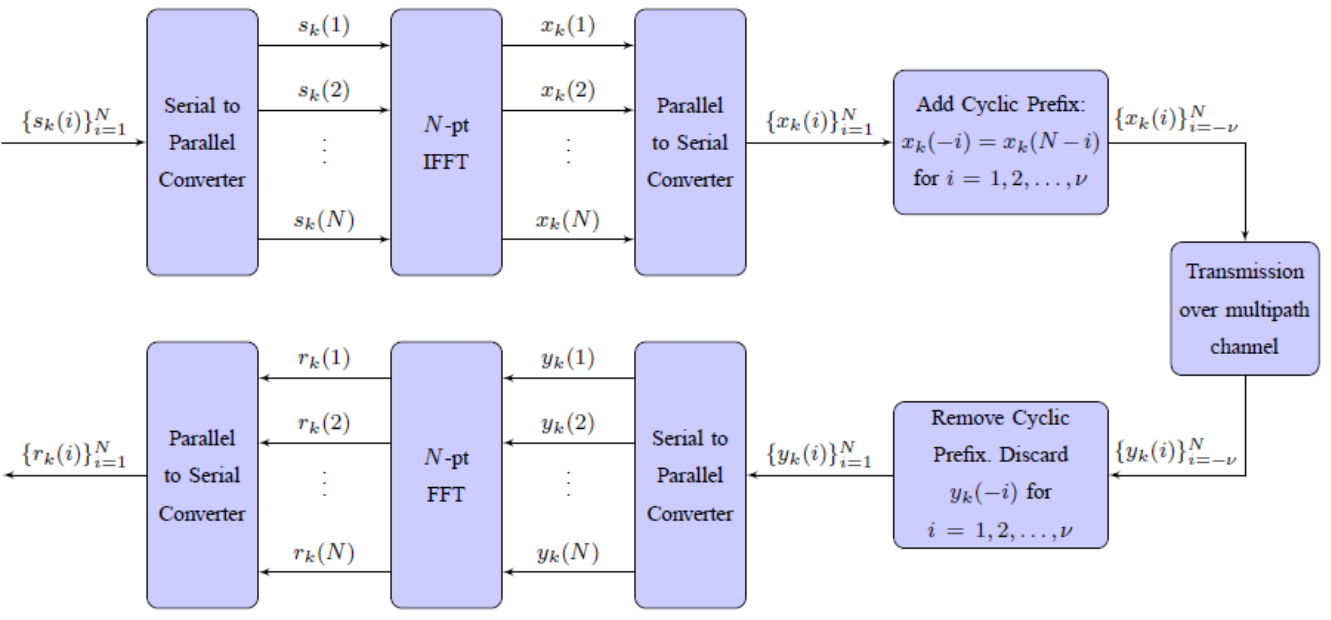
\includegraphics[width=15 cm]{ofdmfig.png}
\caption{System diagram for OFDM (from M. D. Nisar tutorial from OFDM Wiki)}\label{ofdmfig}
\end{center}
\end{figure}

The system includes four blocks making up the sending side, a channel (which is not really
part of the system), and another four blocks on the reciever side which correspond one-to-one
with the blocks on the sending side. The first block on the sending side (and the last on the
receiving side) separates (merges together) the digital signal into (from) N sub-signals. This
block can be described as a serial-to-parallel (parallel-to-serial) converter.

The next block is the inverse discrete Fourier transform, which spreads each symbol out over
the whole length of the combined block. Each signal is now confined to its own separate
sub-band. The separate signals are then combined together again using a parallel to serial
converter. The receiver side carries out these steps in reverse.

This diagram fails to show where modulation occurs. Modulation is the process of converting
a digital signal into an analog signal, often in a frequency band all of which is much higher
than zero. For example, Wifi systems are usually confined to either 2.4-2.4835 GHz or 4.9–
5.85 GHz. In some treatments modulation is regarded as occurring prior to the IFFT, and in
others it is placed just ahead of the channel.

In a sense, part of the modulation process occurs in each of these places. After the parallel to
serial conversion the digital signal is interpreted as complex numbers in the same manner as
after a modulation scheme. These complex numbers pass through the inverse discrete Fourier
transform. Then, in order for the digital signal to be clocked onto the transmission system,
another form of modulation will be needed, which may be little more than digital to analog
conversion.


% \section{Other Methods of Access Sharing}

\section{Concluding Discussion}

By far the most important access control technique that is used in wireless LANs is
CSMA/CA. As discussed in Section \ref{sharingasnoise}, this technique builds on a
completely natural sharing method that applies without (to a large degree) any
technology at all -- sharing by treating other devices as noise. These two methods
work well together. They complement each other.

Other methods of sharing spectrum have also been developed. In particular, sharing
by means of DSSS codes is very effective in its use of power, and in some cases
will probably be more efficient, in its use of spectrum, than CSMA/CA.

